The phase coverage determines the proportion of the program where phase behavior has been defined. Periods of execution where phase behavior has not been defined is considered to be phase transition periods. The phase coverage determines the percentage of the application that can benefit from some client-side optimization and so ideally a high level of phase coverage is preferable. 

Figure~\ref{fig:phasecycles} shows that the phase coverage is not very well behaved with respect to the interval size. That is, as the interval size increases, there is no clear trend in phase coverage. By contrast, there does appear to be some consistent trends for phase coverage with respect to the threshold and model. A higher threshold appears to increase the phase coverage. CPI followed closely by ITD also appears to have higher phase coverage compared to IWS and BBV, with IWS generally having the lowest phase coverage. As far as configuration clients are concerned, adjusting the model as well as increasing the similarity threshold should effectively increase the phase coverage.

\begin{figure}[htbp]
  \begin{center}
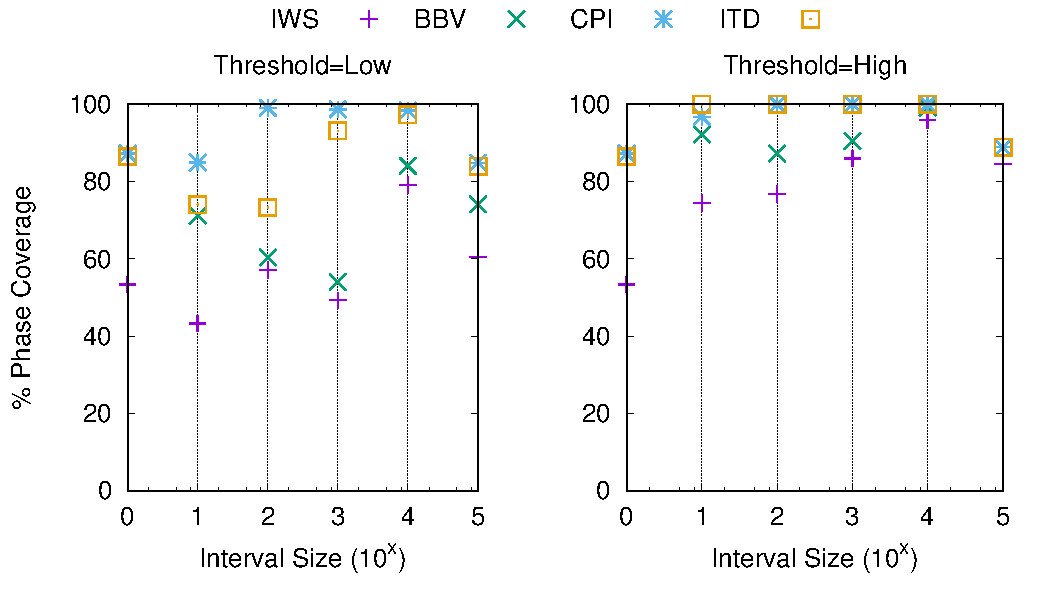
\includegraphics[width=0.99\columnwidth]{figs/phasecyclesthreshold}
  \end{center}
  \caption{Increasing the similarity threshold and using particular models (such as ITD) will tend to result in higher phase coverage.}
  \label{fig:phasecycles}
\end{figure}
